\chapter{Ультрафиолетовые расходимости и суперсимметрическое средство их устранения}

\lectureoverview{Прежде чем вводить формальную математику суперсимметрии, следует точно определить проблему, которую она призвана решить. Мы опишем ультрафиолетовые расходимости как в координатном, так и в импульсном пространстве, с помощью размерностного анализа выведем короткодистанционное поведение скалярного и фермионного пропагаторов и оценим ведущие петлевые поправки к массе скаляра. Скалярная петля и фермионная петля имеют одну и ту же квадратичную зависимость от обрезания, но противоположные знаки. Суперсимметрия становится особенно убедительной, когда мы спрашиваем, какой принцип мог бы обеспечить достаточное совпадение их констант связи, кратностей и масс, чтобы это сокращение было структурным, а не случайным.}

\section{Почему мы вновь возвращаемся к расходимостям?}

Предполагалось сразу перейти к формальному аппарату суперсимметрии. Однако лучше на одну лекцию отложить этот абстрактный материал и заново выстроить мотивацию. Предыдущее обсуждение расходимостей и перенормировки массы прошло слишком быстро, и суперсимметрия будет казаться произвольным математическим изобретением, если мы сначала не увидим в точности, что именно требуется исправить.

Диаграммы Фейнмана входят в физику частиц двумя тесно связанными способами. Наиболее привычным образом они организуют амплитуды рассеяния. Мы задаём входящие и исходящие частицы и суммируем амплитуды, представленные всеми диаграммами требуемого порядка. Они также организуют построение \emph{эффективного лагранжиана}. Здесь слово ``эффективный'' — не похвала в смысле необычайной успешности. Оно означает, что описание является приближённым: недоступные короткодистанционные детали исключены, то есть проинтегрированы, а их влияние закодировано в параметрах и взаимодействиях, которые остаются.

У всякого такого описания есть область применимости. Мы можем задать эту область либо минимальным надёжным расстоянием, обозначаемым здесь \(\delta\), либо максимальным надёжным импульсом,
\begin{equation}
\Lambda\sim \delta^{-1}.
\end{equation}
Эти два обрезания не являются независимыми предположениями. Это фурье-двойственные описания одного и того же ультрафиолетового предела.

\section{Один пропагатор, два описания}

Пропагатор — это амплитуда создания или вставки частицы в одной точке пространства-времени и её уничтожения или обнаружения в другой. Обозначим эти две точки как \(x^\mu\) и \(y^\mu\), а их разделение запишем в виде
\begin{equation}
\Delta^\mu=y^\mu-x^\mu.
\end{equation}
Строчный символ \(\delta\) мы резервируем для обрезания, чтобы не путать разделение и регуляризатор.

Инвариантность относительно переносов означает, что свободный пропагатор зависит от \(x\) и \(y\) только через \(\Delta\). Тот же объект можно преобразовать по Фурье:
\begin{equation}
G(\Delta)
=\int\frac{d^4k}{(2\pi)^4}\,e^{-ik\cdot\Delta}\,\widetilde G(k).
\end{equation}

Когда аудитории задают вопрос ``Какие величины фурье-сопряжены положению?'', ответ — импульс. Следовательно, описание петли в координатном пространстве как пропагатора, возвращающегося в исходную точку, эквивалентно описанию в импульсном пространстве как интеграла по всем импульсам, которые могут циркулировать по петле. Правила в импульсном пространстве требуют налагать сохранение импульса в каждой вершине; координатное пространство делает нынешний аргумент степенного счёта более наглядным.

Эта эквивалентность выявляет ультрафиолетовую проблему ещё до всяких вычислений. В координатном пространстве петля исследует предел совпадающих точек \(\Delta\to0\). В импульсном пространстве она исследует предел \(|k|\to\infty\). Большой импульс означает малую длину волны, поэтому короткодистанционная сингулярность и высокоимпульсная расходимость — одно и то же явление в разных координатах.

В лекции рассматриваются простейшие спиновые классы: скалярные поля, фермионные поля и, на заднем плане, калибровочные поля. Скаляры имеют спин нуль и представляются однокомпонентным полем \(\phi(x)\). Когда эта лекция записывалась в 2010, бозон Хиггса ещё не был открыт и описывался как главный скаляр, ожидавшийся в физике частиц. Эта историческая ситуация объясняет шутливое выражение ``хиггли-виггли''; поле было физически крайне важным, но ещё не было экспериментально подтверждено.

Для вещественного скалярного поля пропагатор можно схематически записать в виде
\begin{equation}
G_\phi(x,y)=\expect{0|T\!\left\{\phi(x)\phi(y)\right\}|0}
=G_\phi(\Delta).
\end{equation}
Соглашение о временном упорядочении и нормировка не будут важны для нашего степенного счёта. Существенно то, что два вставления поля описывают создание в одной точке и уничтожение в другой.

\begin{classroomqa}
\audiencequestion{Являются ли \(x\) и \(y\) положениями в пространстве или в пространстве-времени? \lecturetimestamp{00:09:31}}
\lecturerresponse{Это точки пространства-времени. Каждая из них является четырёхвектором. Поэтому пропагатор зависит от их четырёхмерного разделения и, в лоренц-инвариантном вакууме, от соответствующего инвариантного интервала.}
\end{classroomqa}

Частица со спином 1/2 описывается полем Дирака \(\psi_i(x)\). Индекс \(i\) — это спинорный индекс, а не пространственная компонента, и поэтому пропагатор является матрицей:
\begin{equation}
S_{ij}(x,y)=\expect{0|T\!\left\{\psi_i(x)\bar\psi_j(y)\right\}|0}
=S_{ij}(\Delta).
\end{equation}

Следующий вопрос аудитории даёт число компонент: четырёхмерное поле Дирака имеет четыре комплексные компоненты. Безмассовое поле Вейля можно описать двумя комплексными компонентами, так что левые и правые поля можно рассматривать по отдельности. Для нынешнего размерностного рассуждения важно только наличие спинорной матричной структуры.

Поскольку \(S_{ij}\) является \(4\times4\)-матрицей, его можно разложить по базису матриц Дирака. Сначала мы опустим эти индексы и восстановим их, когда они станут необходимы. Это не утверждение, будто матричная структура отсутствует; это намеренное упрощение, пока мы устанавливаем ультрафиолетовый степенной закон.

\begin{classroomqa}
\audiencequestion{Когда в пропагаторе должно появляться сопряжённое, то есть эрмитово-сопряжённое, поле? \lecturetimestamp{00:14:06}}
\lecturerresponse{Для вещественного нейтрального скаляра в этом схематическом обсуждении одно и то же поле содержит операторы рождения и уничтожения, так что отдельное эрмитово-сопряжённое поле не требуется. Для заряженного поля необходимо различать операторы частицы и античастицы. Поэтому \(\psi\), \(\psi^\dagger\) и, ковариантно, \(\bar\psi=\psi^\dagger\gamma^0\) для электрона играют разные роли.}
\end{classroomqa}

Физическая частица Хиггса нейтральна, хотя лежащее в основе Стандартной модели поле Хиггса является электрослабым дублетом. В лекции в качестве локальной модели используется вещественный нейтральный скаляр; этого упрощения достаточно для ультрафиолетовой оценки.\editorialnote{Это различие не позволяет принять схематический пример вещественного скаляра за полное утверждение об электрослабом мультиплете Хиггса.}

\section{Естественные единицы и размерность скалярного поля}

Положим \(\hbar=c=1\). Тогда длина и время имеют одинаковую размерность, тогда как энергия, масса и импульс имеют размерность обратной длины:
\begin{equation}
[m]=[E]=[p]=L^{-1}.
\end{equation}
Действие входит в фазу \(e^{iS}\), поэтому оно безразмерно. Типичное скалярное действие в четырёх измерениях пространства-времени имеет вид
\begin{equation}
S_\phi=\int d^4x\left[
\frac12\partial_\mu\phi\,\partial^\mu\phi
-\frac12m^2\phi^2
-\frac{\lambda}{4!}\phi^4
+\cdots\right].
\end{equation}
Обычные множители \(1/2\) и \(1/4!\) не влияют на размерностный анализ.

Начнём с кинетического члена. Поскольку \([d^4x]=L^4\) и \([\partial_\mu]=L^{-1}\), из условия безразмерности получаем
\begin{align}
1
&=L^4\left(L^{-1}[\phi]\right)^2,\\
[\phi]&=L^{-1}.
\end{align}
Массовый член даёт проверку:
\begin{equation}
L^4[m^2][\phi^2]
=L^4L^{-2}L^{-2}=1.
\end{equation}

Следующий вопрос аудитории касается размерности квартической константы связи. В четырёх измерениях пространства-времени она безразмерна:
\begin{equation}
L^4[\lambda][\phi]^4=L^4[\lambda]L^{-4}=1
\quad\Longrightarrow\quad [\lambda]=L^0.
\end{equation}
Это делает взаимодействие \(\phi^4\) особым в четырёх измерениях. Размерности \(\phi^6\) и взаимодействий более высокого порядка следуют из того же правила, но их константы связи содержат отрицательные степени массы и потому указывают на более ограниченную роль в эффективной теории.

Таким образом, уже размерности полей говорят нам, какие взаимодействия могут появляться с безразмерными коэффициентами. Тем же методом мы определим оба пропагатора и юкавскую константу связи, не вычисляя детально какой-либо интеграл Фейнмана.

\section{Скалярный пропагатор на малых расстояниях}

Сначала рассмотрим безмассовый скаляр. Собственного масштаба длины нет, так что единственный доступный масштаб — это разделение \(\Delta\). Инвариантность относительно переносов оставляет только \(\Delta\), лоренц-инвариантность сводит зависимость к его инвариантной величине, а произведение двух скалярных полей имеет размерность \(L^{-2}\). С точностью до численного множителя,
\begin{equation}
G_0(\Delta)\sim\frac{1}{\Delta^2}.
\end{equation}
Множители вроде \(4\pi^2\) нельзя определить одним лишь размерностным рассуждением.

Масса вводит комптоновскую длину \(m^{-1}\). Её влияние легче всего понять из соотношения дисперсии
\begin{equation}
E=\sqrt{\bm p^{,2}+m^2},
\qquad
E=|\bm p|\quad(m=0).
\end{equation}
При \(|\bm p|\gg m\) массой можно пренебречь. Поскольку большой импульс исследует малые расстояния, массивный пропагатор должен переходить в безмассовое поведение \(1/\Delta^2\) при \(\Delta\to0\). На расстояниях, гораздо больших \(m^{-1}\), распространение подавлено. В лекции этот факт схематически выражается как
\begin{equation}
G_m(\Delta)\sim \frac{e^{-m|\Delta|}}{\Delta^2}.
\end{equation}
Это намеренно не точная формула. В четырёхмерном евклидовом пространстве точный свободный пропагатор пропорционален \(mK_1(mr)/r\), где \(r=|\Delta|\); он имеет ту же ультрафиолетовую сингулярность \(1/r^2\) и экспоненциальное затухание на больших расстояниях, сопровождаемое степенным предмножителем.\editorialnote{Форма с функцией Бесселя даёт стандартное точное завершение схематической экспоненты из лекции и не требуется для её аргумента степенного счёта.}

Ключевой вывод прост: масса ослабляет распространение на больших расстояниях, но не устраняет сингулярность при совпадении точек. Достаточно близко к точке любая конечная масса становится несущественной.

\section{Скалярная диаграмма-головастик и тонкая подстройка}

Квартическое взаимодействие \(\lambda\phi^4\) даёт вершину с четырьмя линиями. Соедините две её линии друг с другом и оставьте две внешние скалярные линии. Получающаяся диаграмма-головастик исправляет коэффициент при \(\phi^2\), а значит, и квадрат массы скаляра.

Сохранённый кадр фиксирует точный переход от размерностного анализа к этой петлевой поправке. Слева по-прежнему видно дисперсионное соотношение, справа всё ещё частично видны скалярное действие и размерность поля, а в центре только что появилась маленькая диаграмма-головастик.

\begin{figure}[H]
\centering
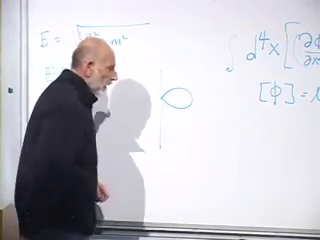
\includegraphics[width=0.72\textwidth]{lecture_03_figure_02.png}
\lectureframe{00:28:30.560}

\medskip
\begin{tikzpicture}[line width=0.8pt,scale=1.0]
  \draw[dashed] (-2.6,0) -- (0,0) -- (2.6,0);
  \fill (0,0) circle (0.055);
  \draw (0,0) .. controls (-0.85,0.7) and (-0.85,1.6) .. (0,1.6)
                .. controls (0.85,1.6) and (0.85,0.7) .. (0,0);
\end{tikzpicture}
\caption{Доска в момент перехода к скалярной самоэнергии, а затем — осторожная схематическая перерисовка топологии головастика. На снимке экрана достоверно видны петля, релятивистская и безмассовая формулы для энергии, а также часть действия; не утверждается, что заслонённые коэффициенты и обозначения различимы.}
\end{figure}

В вершине скаляр может быть поглощён и затем вновь испущен, тогда как две другие линии распространяются из точки обратно в неё саму. С точностью до численных и комбинаторных множителей поправка равна
\begin{equation}
\delta m_\phi^2\sim \lambda G_\phi(0).
\end{equation}
Пропагатор при совпадающих точках бесконечен в континуальном приближении. Эффективная теория не претендует на применимость на сколь угодно малых расстояниях, поэтому наложим \(|\Delta|\geq\delta\). Тогда
\begin{equation}
G_\phi(0)\longrightarrow G_\phi(\delta)sim\frac{1}{\delta^2},
\qquad
\delta m_\phi^2\sim\frac{\lambda}{\delta^2}sim\lambda\Lambda^2.
\end{equation}
Расходимость называется квадратичной, поскольку содержит две степени импульсного обрезания. Интегрирование в пространстве импульсов приводит к тому же выводу: чрезмерный вклад дают сколь угодно большие петлевые импульсы. Не меняет диагноза эффективной теории и то, определяется ли в конечном счёте кратчайший масштаб великим объединением, квантовой гравитацией или чем-то ещё, пока невообразимым.

Это проблема тонкой подстройки. Если \(\delta\) чрезвычайно мало, а \(\lambda\) не исключительно мало, радиационная поправка намного больше квадрата массы скаляра, наблюдаемого при низких энергиях. Голый коэффициент и петлевая поправка должны тогда взаимно компенсироваться вплоть до неправдоподобно большого числа знаков:
\begin{equation}
m_{\mathrm{physical}}^2
=m_{\mathrm{bare}}^2+\delta m_\phi^2.
\end{equation}
Массивный пропагатор не спасает положения. На расстояниях, ответственных за расходимость, \(e^{-m|\Delta|}\simeq1\). Ультрафиолетовая петля забывает о массе ещё задолго до достижения обрезания.

\section{Размерности фермионов и их пропагатор}

Теперь повторим тот же размерностный анализ для дираковского фермиона. Его свободное действие имеет вид
\begin{equation}
S_\psi=\int d^4x\,
\bar\psi\left(i\gamma^\mu\partial_\mu-m\right)\psi.
\end{equation}
Гамма-матрицы являются числовыми и безразмерными. Кинетический член содержит только одну производную, поэтому
\begin{align}
1
&=L^4[\bar\psi]L^{-1}[\psi],\\
[\psi]=[\bar\psi]&=L^{-3/2}.
\end{align}
Полуцелые степени не должны пугать; фермионы привносят половинки во многих местах.

\begin{classroomqa}
\audiencequestion{Не проще ли вывести \([\psi]\) из массового члена? \lecturetimestamp{00:36:02}}
\lecturerresponse{Да. Массовый член даёт \(L^4L^{-1}[\bar\psi\psi]=1\), следовательно, \([\bar\psi\psi]=L^{-3}\) и \([\psi]=L^{-3/2}\). Сначала был использован вывод из кинетического члена, потому что он остаётся осмысленным в безмассовой теории и показывает, почему масса фермиона входит как \(m\), а не \(m^2\).}
\end{classroomqa}

Два фермионных поля имеют размерность \(L^{-3}\), поэтому компактная размерностная запись лекции для безмассового пропагатора такова:
\begin{equation}
S(\Delta)\sim\frac{1}{|\Delta|^3}.
\end{equation}
Восстановление его матричной структуры даёт более точный числитель, требуемый лоренц-ковариантностью:
\begin{equation}
S_{ij}(\Delta)
\propto
\frac{\left(\gamma_\mu\Delta^\mu\right)_{ij}}
{\left(\Delta^2\right)^2}.
\end{equation}
Числитель добавляет одну степень длины, и потому знаменатель содержит четыре степени интервала; итоговая размерность остаётся \(L^{-3}\). Как и в скалярном случае, масса фермиона подавляет пропагатор при большом разделении, но не меняет этого короткодистанционного масштабирования.

\section{Почему замкнутая фермионная петля даёт знак минус}

Теперь можно спросить, может ли фермионная диаграмма скомпенсировать проблемный бозонный вклад в самоэнергию. Скалярная диаграмма-головастик имеет положительный знак, с точностью до положительных численных множителей, таких как степени \(\pi\) и комбинаторные коэффициенты. Замкнутая фермионная петля несёт противоположный знак.

\begin{classroomqa}
\audiencequestion{Связан ли знак минус у фермионной петли с прежним обсуждением одного полного поворота? \lecturetimestamp{00:40:21}}
\lecturerresponse{Он относится к той же фермионной знаковой структуре, но удобное доказательство здесь опирается на антисимметрию при обмене, а не на геометрическую ориентацию петли. Разрежьте две петли, обменяйте тождественные частицы и снова соедините. Обмен превращает две петли в одну и даёт знак минус только для фермионов.}
\end{classroomqa}

Этот аргумент стоит изложить полностью. Предположим, что однопетлевая диаграмма имеет знак \(\sigma\), то есть либо плюс, либо минус. Две несвязанные тождественные петли имеют знак
\begin{equation}
\sigma^2=+1.
\end{equation}
Разрежем обе петли одновременно. Теперь между разрезами распространяются две тождественные частицы. Их обычная двухчастичная волновая функция симметрична для бозонов и антисимметрична для фермионов:
\begin{align}
\Psi_B(x_1,x_2)&=+\Psi_B(x_2,x_1),\\
\Psi_F(x_1,x_2)&=-\Psi_F(x_2,x_1).
\end{align}
Антисимметрия также объясняет принцип Паули: если оба фермиона помещены в одно и то же состояние, перестановка физически ничего не меняет, но должна обратить волновую функцию в противоположную, вынуждая её обращаться в нуль.

Снова соедините разрезанные линии после обмена двух частиц. Топологически две петли превратились в одну. Амплитуда с двумя петлями без обмена была положительной. Обмен оставляет её положительной для бозонов и меняет знак для фермионов. Поэтому
\begin{equation}
\begin{aligned}
\operatorname{sign}(\text{closed boson loop})&=+1,\\
\operatorname{sign}(\text{closed fermion loop})&=-1.
\end{aligned}
\end{equation}
Этот вывод общий: каждая независимая замкнутая фермионная петля даёт множитель \(-1\).

\section{Юкавская петля}

Вернёмся к массе скаляра. Бозон не может превратиться в один фермион, потому что тогда изменилась бы чётность числа фермионов. Простейшая фермионная поправка состоит в том, что скаляр расщепляется на фермион-антифермионную пару, которые распространяются по петле и вновь рекомбинируют. Взаимодействие задаётся юкавской связью,
\begin{equation}
\mathcal L_Y=-g\phi\bar\psi\psi.
\end{equation}
Для Хиггса фермионами могут быть кварки или лептоны. Имеются две точки взаимодействия и, следовательно, два множителя \(g\).

В скалярной диаграмме-головастике была одна точка, общее положение которой можно было зафиксировать, поскольку трансляционная инвариантность лишь даёт множитель объёма пространства-времени. В юкавской петле участвуют две точки. Можно зафиксировать одну из них или, что эквивалентно, их среднее положение, но нужно проинтегрировать по их относительному смещению \(\Delta\). Каждый фермионный пропагатор вносит короткодистанционный множитель \(1/|\Delta|^3\), поэтому
\begin{equation}
\delta m_{\phi,F}^2
\sim
-g^2\int_{|\Delta|\geq\delta}d^4\Delta\,
\frac{1}{|\Delta|^6}.
\end{equation}

После того как записаны два пропагатора, интеграл по разделению и две константы связи, остаётся спросить у аудитории ещё об одном последнем множителе. Ответ — знак минус. Два пропагатора замыкаются в фермионную петлю, поэтому весь этот в остальном положительный короткодистанционный интеграл умножается на \(-1\).

Размерностный анализ уже определяет расходимость. Четыре степени длины приходят из \(d^4\Delta\), шесть стоят в знаменателе, и единственным оставшимся масштабом длины остаётся обрезание:
\begin{equation}
\int_{|\Delta|\geq\delta}
\frac{d^4\Delta}{|\Delta|^6}
\sim\frac{1}{\delta^2}.
\end{equation}
В четырёхмерных евклидовых радиальных координатах это можно записать явно:
\begin{equation}
\int_{\delta}^{R}d^4\Delta\,\frac{1}{|\Delta|^6}
=2\pi^2\int_{\delta}^{R}dr\,\frac{r^3}{r^6}
=\pi^2\left(\frac{1}{\delta^2}-\frac{1}{R^2}\right).
\end{equation}
Следы по спинорам и нормировки пропагаторов меняют коэффициент, но не квадратичную степень обрезания.\editorialnote{Радиальный интеграл — это стандартная явная версия размерностной оценки, сделанной на лекции. Он записан через евклидово расстояние, где наглядны положительность и ультрафиолетовый подсчёт степеней.}

\begin{classroomqa}
\audiencequestion{Может ли изменение порядка или выбор пределов интегрирования изменить знак? \lecturetimestamp{00:51:06}}
\lecturerresponse{Нет. Это не одномерный ориентированный интеграл, в котором пределы порождают физический знак. Это интеграл по четырём компонентам или, ещё яснее, по положительной радиальной мере. Его ультрафиолетовая величина положительна. Отрицательный вклад возникает исключительно из замкнутой фермионной петли.}
\end{classroomqa}

\begin{classroomqa}
\audiencequestion{Какова размерность юкавской константы связи \(g\)? \lecturetimestamp{00:51:51}}
\lecturerresponse{В четырёх измерениях она безразмерна. Поскольку \([\phi]=L^{-1}\) и \([\bar\psi\psi]=L^{-3}\), произведение \(\phi\bar\psi\psi\) имеет размерность \(L^{-4}\), которая в точности компенсируется \(d^4x\).}
\end{classroomqa}

Следовательно, ведущая фермионная поправка имеет вид
\begin{equation}
\delta m_{\phi,F}^2
\sim -C_F\frac{g^2}{\delta^2}
=-C_Fg^2\Lambda^2,
\end{equation}
где \(C_F>0\) содержит численные, спиновые и кратностные множители. Соответствующая скалярная петля имеет вид
\begin{equation}
\delta m_{\phi,B}^2
\sim+C_B\frac{\lambda}{\delta^2}
=+C_B\lambda\Lambda^2.
\end{equation}
Мы ещё не решили проблему тонкой подстройки, но нашли нечто необходимое: вклад с той же степенью ультрафиолетовой расходимости и противоположным знаком.

\section{Что требуется для компенсации}

Было бы чрезвычайной случайностью, если бы не связанные между собой константы связи случайно удовлетворяли
\begin{equation}
C_B\lambda=C_Fg^2
\end{equation}
именно с той точностью, которую требует большая иерархия масштабов. В лекции это сокращённо записывается как \(g^2=\lambda\), при этом опущены зависящие от соглашений и кратностные множители. Для подлинного решения нужна математическая структура, которая навязывает это соотношение, а не просто допускает его.

В этом и состоит суперсимметрический мотив. Суперсимметрия связывает бозоны и фермионы и ограничивает их константы связи такими комбинациями, при которых сокращаются многие иначе опасные расходящиеся члены. Тогда это сокращение воспроизводится от диаграммы к диаграмме, поскольку следует из симметрии, а не потому, что параметры подгоняются по одной петле за раз.

Согласование масс тоже важно. Если массы бозона и фермиона совпадают, их полные пропагаторы можно сопоставить наиболее точно. Если массы немного различаются, полные конечные результаты не сокращаются в точности, потому что пропагаторы различаются на расстояниях, сравнимых с их комптоновскими длинами волн. Тем не менее их общая асимптотика на малых расстояниях может взаимно уничтожить расходящуюся часть:
\begin{equation}
\mathcal I_B(\Delta)-\mathcal I_F(\Delta)
\quad\hbox{may be finite as}\quad \Delta\to0,
\end{equation}
где \(\mathcal I_B\) и \(\mathcal I_F\) обозначают полные бозонное и фермионное подынтегральные выражения петлевого интеграла после учета вершин, числителей и кратностей. Сами пропагаторы имеют разные размерности и непосредственно друг из друга не вычитаются. Даже когда ультрафиолетовые члены сокращаются, может остаться конечный остаток. Здесь и возникает возможность приближённой или нарушенной суперсимметрии. Точное равенство даёт наиболее чистое сокращение; достаточно контролируемое нарушение всё ещё может устранить ультрафиолетовую катастрофу, оставив наблюдаемые расщепления масс.

Таким образом, мы пришли к суперсимметрии, ещё не записав её алгебру. Цепочка рассуждений завершена:
\begin{equation}
\begin{gathered}
G_\phi(\Delta)\sim \Delta^{-2},
\qquad
\delta m_{\phi,B}^2\sim+C_B\lambda\Lambda^2,\\[0.4em]
S_\psi(\Delta)\sim \Delta^{-3},
\qquad
\delta m_{\phi,F}^2\sim-C_Fg^2\Lambda^2,\\[0.4em]
\text{symmetry-enforced matching}\\
\Longrightarrow\quad
\text{quadratic divergences cancel}.
\end{gathered}
\end{equation}
Следующая задача — понять абстрактный принцип симметрии, который обеспечивает выполнение этих соотношений, и рассмотреть конкретные примеры его действия.